%% arara directives
% arara: xelatex
% arara: bibtex
% arara: xelatex
% arara: xelatex
\documentclass[twocolumn]{article} % Method A for two-column formatting

\usepackage{preprint}
\usepackage{glossaries}
\usepackage{graphicx}
\usepackage{enumitem}
\setlist[itemize]{leftmargin=1.5em} % custom indentation
\setlist[enumerate]{leftmargin=1.5em} % for numbered lists

%% Math packages
\usepackage{amsmath, amsthm, amssymb, amsfonts}

%% Algorithm packages
\usepackage{algorithm}
\usepackage{algpseudocode}

%% Bibliography options
\usepackage[numbers,square]{natbib}
\bibliographystyle{unsrtnat}
%\usepackage{natbib}
%\bibliographystyle{Geology}

%% General packages
\usepackage[utf8]{inputenc}	% allow utf-8 input
\usepackage[T1]{fontenc}	% use 8-bit T1 fonts
\usepackage{xcolor}		% colors for hyperlinks
\usepackage[colorlinks = true,
            linkcolor = purple,
            urlcolor  = blue,
            citecolor = cyan,
            anchorcolor = black]{hyperref}	% Color links to references, figures, etc.
\usepackage{booktabs} 		% professional-quality tables
\usepackage{multirow}		% multi-row cells in tables
\usepackage{nicefrac}		% compact symbols for 1/2, etc.
\usepackage{microtype}		% microtypography
\usepackage{lineno}		% Line numbers
\usepackage{float}			% Allows for figures within multicol
%\usepackage{multicol}		% Multiple columns (Method B)

\usepackage{lipsum}		%  Filler text

 %% Special figure caption options
\usepackage{newfloat}
\DeclareFloatingEnvironment[name={Supplementary Figure}]{suppfigure}
\usepackage{sidecap}
\sidecaptionvpos{figure}{c}

% Section title spacing  options
\usepackage{titlesec}
\titlespacing\section{0pt}{12pt plus 3pt minus 3pt}{1pt plus 1pt minus 1pt}
\titlespacing\subsection{0pt}{10pt plus 3pt minus 3pt}{1pt plus 1pt minus 1pt}
\titlespacing\subsubsection{0pt}{8pt plus 3pt minus 3pt}{1pt plus 1pt minus 1pt}

% Fix for fancyhdr \headheight warning
\setlength{\headheight}{12pt}

% ORCiD insertion
\usepackage{tikz,xcolor,hyperref}

\definecolor{lime}{HTML}{A6CE39}
\DeclareRobustCommand{\orcidicon}{
	
\begin{tikzpicture}
	\draw[lime, fill=lime] (0,0) 
	circle [radius=0.16] 
	node[white] {{\fontfamily{qag}\selectfont \tiny ID}};
	\draw[white, fill=white] (-0.0625,0.095) 
	circle [radius=0.007];
	\end{tikzpicture}
	\hspace{-2mm}
}
\foreach \x in {A, ..., Z}{\expandafter\xdef\csname orcid\x\endcsname{\noexpand\href{https://orcid.org/\csname orcidauthor\x\endcsname}
			{\noexpand\orcidicon}}
}
% Define the ORCID iD command for each author separately. Here done for two authors.
\newcommand{\orcidauthorA}{0009-0004-5890-4819}
% \newcommand{\orcidauthorB}{0009-0006-4869-9705}
\newacronym{vit}{ViT}{Vision Transformer}
\newacronym{kiva}{KiVA}{Kid-inspired Visual Analogies}

\makeglossaries

%%%%%%%%%%%%%%%%   Title   %%%%%%%%%%%%%%%%
\date{October 7, 2025}
\title{A ViT-based Siamese Network for Visual Reasoning in the KiVA Challenge }
\shorttitle{}

%%%%%%%%%%%%%%%  Author list  %%%%%%%%%%%%%%%
\usepackage{authblk}
\renewcommand*{\Authfont}{\bfseries}
\author[1]{Joan Salvà Soler*\orcidA{}} 

\affil[1]{H2O.ai}

%%%%%%%%%%%%%%    Front matter    %%%%%%%%%%%%%%
\begin{document}

\twocolumn[ % Method A for two-column formatting
  
\maketitle

\begin{abstract}
We present a novel \gls{vit}-based Siamese network for visual analogical reasoning developed for the \gls{kiva} Challenge. This architecture achieves 95.9\% accuracy on the benchmark, demonstrating strong performance across all difficulty levels and establishing the effectiveness of the architecture for visual reasoning tasks. Code is available at \url{https://github.com/jsalvasoler/kiva-iccv}.

\end{abstract} 

\vspace{0.35cm}

] % Method A for two-column formatting


%%%%%%%%%%%%%%%  Main text   %%%%%%%%%%%%%%%
% \linenumbers

\section{Introduction}

Visual analogical reasoning, the ability to infer and apply abstract rules from visual examples, is a hallmark of human intelligence and a critical component of flexible, general-purpose problem-solving \cite{gentner1983}. The KiVA benchmark provides a framework for evaluating this capability in AI systems, grounding the task in developmental psychology by using simple transformations of everyday objects that are solvable even by young children \cite{yee2025kiva}. The challenge frames this task in the classic A:B :: C:? format, where a model must identify the transformation that turns A into B and apply it to C to find the correct outcome among several choices. The following is an example of a task:

\begin{figure}[h]\vspace{-0.5\baselineskip}
    \centering
    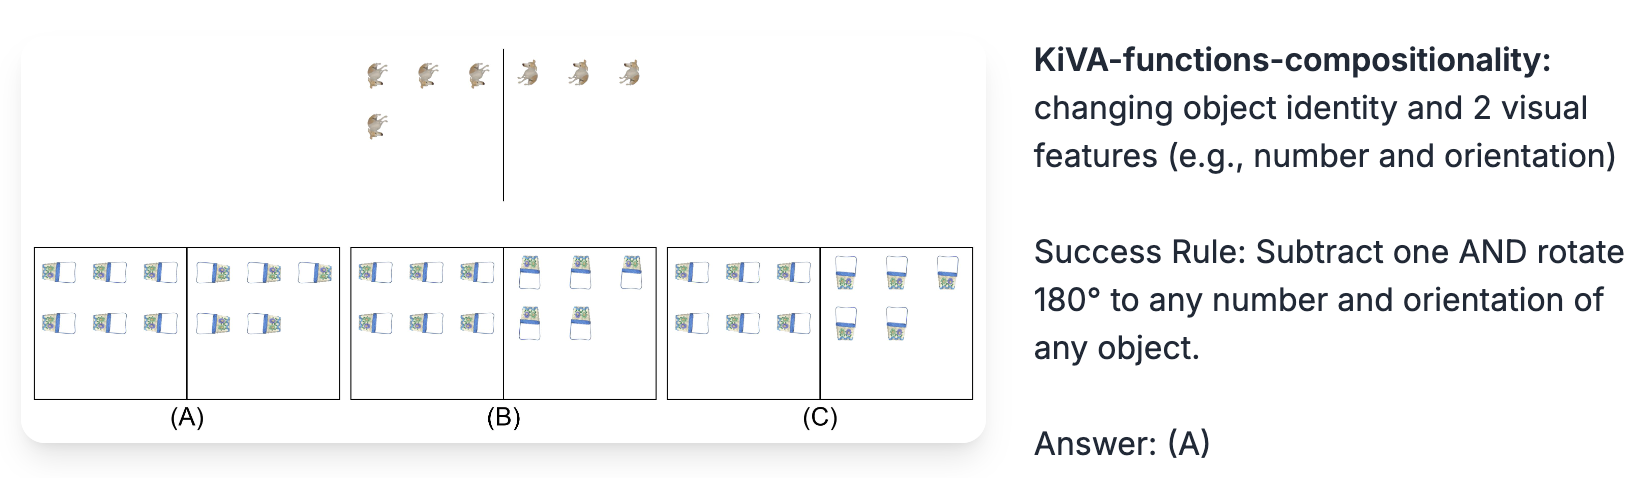
\includegraphics[width=0.5\textwidth]{figures/kiva-example.png}
    \caption{Example of a KiVA task.}
    \label{fig:kiva_example}
\end{figure}\vspace{-0.5\baselineskip}

The KiVA benchmark comprises three difficulty levels: \textbf{KiVA (easy)}, where only the object identity changes between the example and test transformations; \textbf{KiVA-functions (moderate)}, in which both the object identity and one visual feature (such as orientation, size, or number) change; and \textbf{KiVA-functions-compositionality (difficult)}, where the object identity and two visual features (for example, orientation, size, or number) change between the example and test. This progression allows for a systematic evaluation of analogical reasoning as the complexity of the required transformation increases.

\section{Method}

Our approach employs a Siamese Network \cite{Chicco2021SiameseOverview} designed specifically for visual analogical reasoning. Given an example transformation pair ($A$, $B$) and a test scenario $C$ with multiple candidate choices ($D_1, \dots, D_n$), the model must identify which choice correctly completes the analogy. The model operates as follows:
\begin{enumerate}
    \item The example transformation ($A$, $B$) is encoded using a transformation encoder to produce a transformation vector $\mathbf{t}_{\mathrm{AB}}$.
    \item Each candidate transformation $(C, D_1), \ldots, (C, D_n)$ is similarly encoded to produce choice vectors $\mathbf{t}_{\mathrm{CD}_i}$.
    \item The goal is to identify the choice $i$ where $\mathbf{t}_{\mathrm{CD}_i}$ is most similar to $\mathbf{t}_{\mathrm{AB}}$, typically measured using cosine similarity.
\end{enumerate}

An important detail of our approach is that we assume that the eight images of the KiVA task can be extracted from the ``stitched'' image. It is a fair assumption, as the complexity of the task is the same when the images are given separately. Moreover, it would be simple to train a model to extract the images from the stitched image, if necessary. In our KiVA task, with $n=3$, we will refer to these images as $A$, $B$, $C$, $D_1$, $D_2$, $D_3$, where $D_1$, $D_2$, $D_3$ are the three choices. 

\paragraph{Transformation Encoder}

A traditional approach to this task would be to encode each image independently and compute the transformation as \(t = f(B) - f(A)\), following the analogy-making strategy used in models like Word2Vec \cite{mikolov2013efficient}. However, we found that this method was insufficient for capturing the nuanced visual relationships between images in the analogy task. Instead, we model the transformation directly as \(t = f(A, B)\), where $f$ is a transformer-based image encoder that leverages cross-image attention to jointly process both images. Through experiments with various vision transformer architectures (ViT and DINOv3), we determined that a ViT-based approach was the most effective for this purpose.

\paragraph{Architecture of the ViT-based Transformation Encoder}
We adapt the ViT architecture, which is pretrained on 224$\times$224 images, to process two images as a unified sequence. Both input images ($A$ and $B$) are independently passed through the pretrained ViT patch embedding layer. For 224$\times$224 images with 16$\times$16 patches, this produces two sequences of 196 patch embeddings each, with dimension $d$ (e.g., $d=384$ for ViT-Small). These patch embeddings are concatenated and a learnable $[\text{CLS}]$ token is prepended to form a unified sequence that will aggregate the transformation representation. Positional embeddings are then added to provide spatial location information, where the embedding matrix is extended by duplicating the original patch positional embeddings for both images. Learned segment embeddings distinguish patches from the ``before'' image (Segment 1) versus the ``after'' image (Segment 2), with Segment 0 for the $[\text{CLS}]$ token. The sequence is then passed through the pretrained ViT transformer blocks (12 layers for ViT-Small). Critically, the self-attention mechanism allows patches from image $A$ to attend to patches from image $B$, enabling direct comparison of corresponding spatial regions. Finally, after layer normalization, the $[\text{CLS}]$ token is extracted and passed through a learnable projection head (not part of pretrained ViT) consisting of linear layers, ReLU, dropout, and layer normalization to produce the final transformation embedding $\mathbf{t}_{AB}^{\text{final}} \in \mathbb{R}^{e}$.
The complete forward pass can be summarized as:
\begin{align*}
    &\text{patches}_A,\, \text{patches}_B \in \mathbb{R}^{196 \times d} \\
    &x = [\![\text{CLS}]\,;\, \text{patches}_A\,;\, \text{patches}_B] \in \mathbb{R}^{393 \times d} \\
    &x \leftarrow x + [\text{pos}_{\text{CLS}}\,;\, \text{pos}_{\text{patches}}\,;\, \text{pos}_{\text{patches}}] \\
    &x \leftarrow x + \text{segment\_embed}(\text{seg\_ids}) \\
    &x \leftarrow \text{TransformerBlocks}(x) \\
    &\mathbf{t}_{AB}^{\text{final}} = \text{ProjectionHead}(\text{LayerNorm}(x)[0]) \in \mathbb{R}^{e}
\end{align*}

\paragraph{Loss Function}
After comparing the standard triplet loss and softmax cross-entropy loss, we found that a simple \textbf{contrastive analogy loss} \cite{chopra2005learning} performed best. Given a training example consisting of an example transformation $\mathbf{t}_{\text{ex}}$, one correct choice transformation $\mathbf{t}_{\text{pos}}$, and $n$ incorrect choice transformations $\{\mathbf{t}_{\text{neg}_i}\}_{i=1}^{n}$, the loss aims to maximize the similarity between $\mathbf{t}_{\text{ex}}$ and $\mathbf{t}_{\text{pos}}$, minimize the similarity between $\mathbf{t}_{\text{ex}}$ and each $\mathbf{t}_{\text{neg}_i}$, and enforce a margin $m$ between positive and negative similarities:
\begin{equation}
\mathcal{L} = \frac{1}{n-1}\sum_{i=1}^{n-1} \max\left(0, m - \left(s_{\text{pos}} - s_{\text{neg}_i}\right)\right)
\end{equation}
where $s_{\text{pos}} = \text{sim}(\mathbf{t}_{\text{ex}}, \mathbf{t}_{\text{pos}})$ and $s_{\text{neg}_i} = \text{sim}(\mathbf{t}_{\text{ex}}, \mathbf{t}_{\text{neg}_i})$ are the cosine similarities. In the KiVA challenge with $n=3$ choices per example, we have $2$ negative examples.


\section{Experiments \& Results}

\paragraph{Implementation and Hardware} The implementation uses PyTorch for modeling and Neptune for logging. We perform the experiments on a single NVIDIA L40S GPU with $40$GB of memory.

\paragraph{Model Configuration}
We use \texttt{vit\_small\_patch16\_224} as our encoder backbone, initializing its weights with pretrained checkpoints from \texttt{timm}. This sets a resolution of $224 \times 224$ pixels. We set the embedding dimension to $e=512$, and the projection head consists of two linear layers with a ReLU activation, dropout, and layer normalization, mapping the ViT output to the final embedding space. This gives the model a total of $22.7$M learnable parameters.

\paragraph{Training Configuration}
The optimizer AdamW with weight decay $1 \times 10^{-4}$ is used to train the model. 
A cosine annealing schedule is used to decay the learning rate over $20$ total epochs, starting from $3 \times 10^{-5}$ for the encoder parameters and $3 \times 10^{-4}$ for the projection parameters. The batch size is $64$ with a gradient accumulation of $4$ for an effective batch size of $256$. The contrastive margin is $m = 0.05$.
We use mixed precision training to speed up the training process.

\paragraph{Training Data}
We use the code from the official KiVA dataset \cite{yee2025kiva} to augment the provided training data. Our pipeline generated random training samples on-the-fly that follow a similar distribution as the official training set. We included transformations with parameter combinations not present in the original training set to improve model generalization. We set the epoch length to $65536$ examples, $2752$ of which come from the official training set, and the rest are generated on-the-fly.

\paragraph{Results}
Table~\ref{tab:kiva_results} presents our model's Top-1 accuracy on both validation and test sets, broken down by difficulty level. The results demonstrate the effectiveness of our approach, and the model's generalization is excellent, as the gap between validation and test accuracy is minimal. Figure~\ref{fig:radar_plot} provides a granular breakdown of test set performance, showing that while the model performance decreases as task complexity increases, particularly on compositionality tasks involving counting. The final configuration was identified after extensive experimentation (152 runs), as illustrated by the sample of training curves in Figure~\ref{fig:train_runs}.

\begin{table}[!htb]
    \caption{Final accuracy (\%) on the KiVA benchmark. Results are shown for validation and test sets across three difficulty levels.}
    \label{tab:kiva_results}
    \centering
    \setlength{\tabcolsep}{5pt} % Reduce column separation
    \begin{tabular}{lcccc}
        \toprule
        \textbf{Split} & \textbf{KiVA} & \textbf{KiVA-func} & \textbf{KiVA-comp} & \textbf{Overall} \\
        & \textbf{(Easy)} & \textbf{(Moderate)} & \textbf{(Difficult)} & \\
        \midrule
        Validation & 100\% & 100\% & 94\% & 95.4\% \\
        Test & 100\% & 100\% & 95\% & 95.9\% \\
        \bottomrule
    \end{tabular}
\end{table}

\begin{figure}[h]\vspace{-0.5\baselineskip}
    \centering
    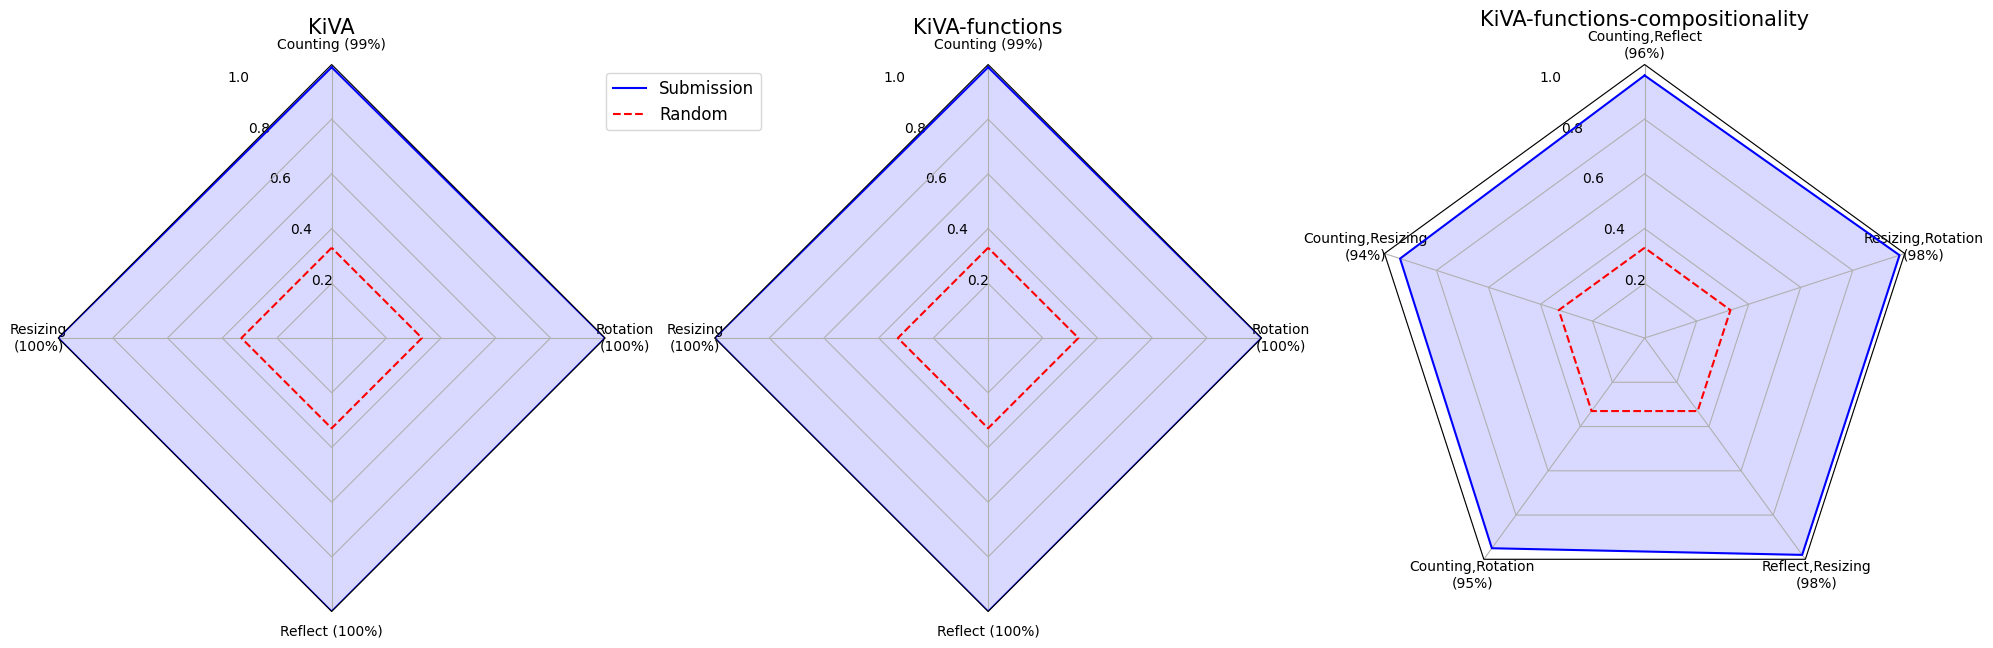
\includegraphics[width=0.5\textwidth]{figures/combined_radar.png}
    \caption{Radar plot of accuracy on the test set by transformation type.}
    \label{fig:radar_plot}
\end{figure}\vspace{-0.5\baselineskip}

\begin{figure}[h]\vspace{-0.5\baselineskip}
    \centering
    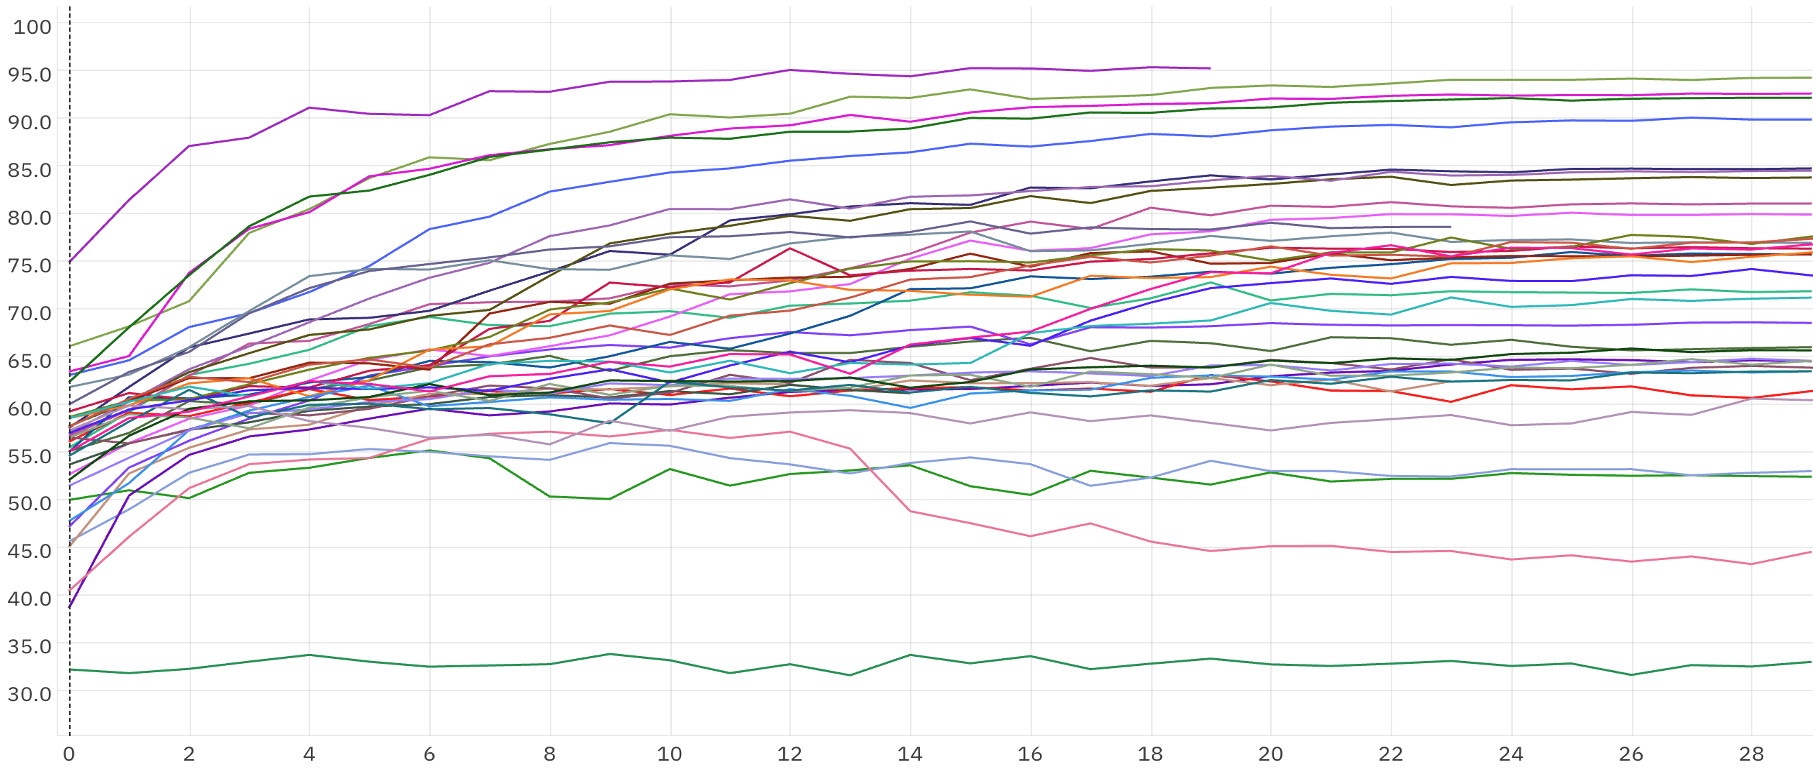
\includegraphics[width=0.5\textwidth]{figures/train_runs.png}
    \caption{Validation accuracy during KiVA training runs.}
    \label{fig:train_runs}
\end{figure}\vspace{-0.5\baselineskip}

\paragraph{Conclusion} We presented a \gls{vit}-based Siamese network that processes image transformation pairs as unified sequences, enabling the direct modeling of visual changes via cross-attention. Our approach achieves 95.9\% accuracy on the \gls{kiva} benchmark, demonstrating that joint encoding of transformation pairs is a highly effective strategy for visual analogical reasoning. This architecture provides a strong foundation for future work on visual reasoning tasks.


%%%%%%%%%%%%%%   Bibliography   %%%%%%%%%%%%%%
\normalsize
\bibliography{references}

\end{document}